

\begin{frame}{\ft{Launching Dialog Windows}}

\doubleFrame{By clicking on links in Re-PDF documents, 
users can launch dialog windows with 
special layout and features.  For 
regular PDF viewers, these links will take users to 
realtors\curlyapos{} web pages.  However, for custom Re-PDF viewers, 
these links will open adjunct viewers --- fine-tuned for 
each realtor --- such as customized dialog boxes 
and 3D or multimedia presentations.}

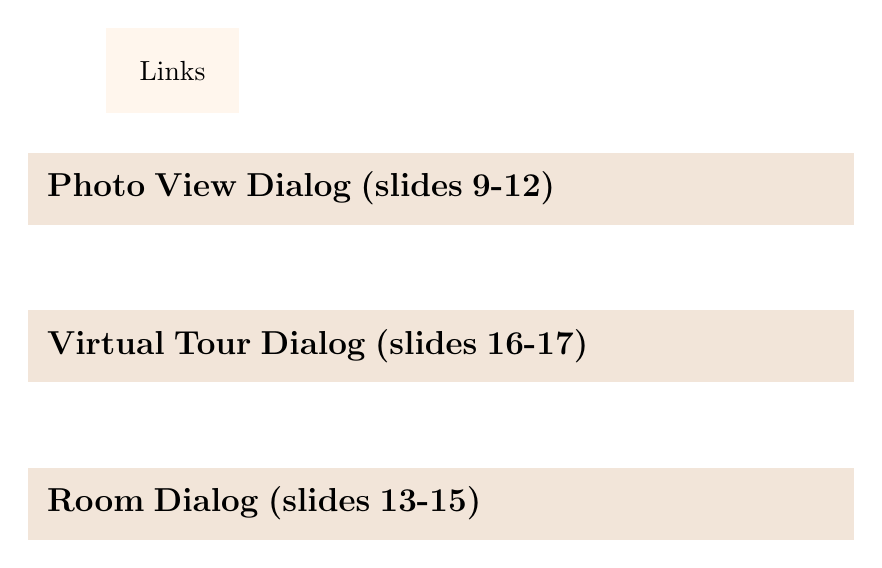
\begin{tikzpicture}
%\nodeincludegraphics[0.87\textwidth]{screenshots/ss-links.png}
\nodeincludegraphicsTR{2.5cm}{2cm}{screenshots/ss-links.png}

\node [anchor=west,fill=orange!8!white,inner sep=12, 
opacity=0.88, text opacity=1] (note) at (9.5,8.5) {\hc{Links}};

%\rectann{darkRed}{0.7}{1mm}{grammarArrowColor}{0.5}{2,8}{5}{-7}{0.5}
\rectanneat{darkRed}{0.7}{1mm}{grammarArrowColor}{0.5}{0,10}{9}{-7}{0.7}

%\draw [-latex, ultra thick, red] (note) to (7, 7);

\colorarr{>=latex, ->}{fcBoxColor!60!black}{0.8}{blGreen!30!red}{1}{1mm}{note}{7, 8}


 \node [anchor=west,fill=brown!20!white,inner sep=7, text width=10cm]
  (longnote) at (8.5,7) {%  %{\color{rb!85!red}{
  {\cframedbox{\large \textbf{Photo View Dialog (slides 9-12)}}}};

\colorarr{>=latex, ->}{fcBoxColor!20!black}
{0.8}{darkRed!70!blue}{2}{1mm}{longnote.west}{6.3, 7.5}


 \node [anchor=west,fill=brown!20!white,inner sep=7, text width=10cm]
  (longnote) at (8.5,5) {%  %{\color{rb!85!red}{
  {\cframedbox{\large \textbf{Virtual Tour Dialog (slides 16-17)}}}};

\colorarr{>=latex, ->}{fcBoxColor!20!black}
{0.8}{darkRed!70!blue}{2}{1mm}{longnote.west}{6.1, 6.8}



 \node [anchor=west,fill=brown!20!white,inner sep=7, text width=10cm]
  (longnote) at (8.5,3) {%  %{\color{rb!85!red}{
  {\cframedbox{\large \textbf{Room Dialog (slides 13-15)}}}};

\colorarr{>=latex, ->}{fcBoxColor!20!black}
{0.8}{darkRed!70!blue}{2}{1mm}{longnote.west}{5.9, 4.7}


%\draw [-latex, draw=darkRed,draw opacity=0.8,line width=#4] #5 to #6;


%[out=120, in=0]
\end{tikzpicture}


\end{frame}

